\section{\texorpdfstring{Reservoir model and controlled\\
dissipator design}{Reservoir model and controlled dissipator design}}
\label{sec:model}

\subsection{The fixed driven reservoir}

We keep the coherent reservoir fixed and change only its coupling to the
environment.
The reservoir is the continuously driven network of \(N\) interacting qubits
introduced in Ref.~\cite{Sannia2024}. During the \(k\)th input interval, a
scalar value \(s_k\in[0,1]\) is held constant for a duration \(\Delta t\), and
the qubits evolve under
\begin{equation}
H(s_k)=\sum_{i<j}J_{ij}\sigma_i^x\sigma_j^x
       +h\sum_i\sigma_i^z+h(1+s_k)\sum_i\sigma_i^x .
\label{eq:hamiltonian}
\end{equation}
The \(J_{ij}\) term couples the qubits, the \(z\) field sets their static
energy scale, and the final term writes \(s_k\) into the transverse drive.
Each reservoir instance uses one sampled set of couplings \(J_{ij}\).
This fixes how the input enters and how information moves before the
environmental organization is varied.

\subsection{\texorpdfstring{Environmental dynamics and\\
reference relaxation}{Environmental dynamics and reference relaxation}}

The Hamiltonian describes isolated evolution, while the environment adds a
second contribution. For the memoryless model used here, the density matrix
obeys the Lindblad master equation
~\cite{Gorini1976,Lindblad1976,BreuerPetruccione2002},
\begin{equation}
\begin{aligned}
\dot{\rho}=\Lind_s(\rho)
 &=-i[H(s),\rho]+\sum_k\D[L_k](\rho),\\
\D[L](\rho)
 &=L\rho L^\dagger-\tfrac12\{L^\dagger L,\rho\}.
\end{aligned}
\label{eq:gkls}
\end{equation}
We use Eq.~\eqref{eq:gkls} as a target engineered GKLS generator, not as the
generic weak-coupling master equation of an arbitrary common bath.
The commutator gives the coherent motion. Each \(\D[L_k]\) describes one
environmental action on average. The operator \(L_k\) identifies the
transition and its coefficient sets the strength. Both parts act continuously.
Because the dissipative term is quadratic in its jump operator,
\[
\D[aL]=\lvert a\rvert^2\D[L],
\]
a coefficient \(\sqrt{\gamma}\) makes \(\gamma\) the corresponding rate
scale.

The standard model gives each qubit its own relaxation channel. Following
Sannia \emph{et al.}~\cite{Sannia2024}, we write
\begin{equation}
L_i=\sqrt{\gamma}\,\sigma_i^-,\qquad i=1,\ldots,N .
\label{eq:sannia}
\end{equation}
The lowering operator \(\sigma_i^-\) maps the excited state of qubit \(i\) to
its ground state. One operator per site gives independent relaxation, while
the common \(\sqrt{\gamma}\) sets the rate. This is \emph{uniform local
relaxation}, the reference point from which we vary environmental
organization.

\subsection{Generator-level dissipator geometry}

The reference process exposes two operational coordinates. A \emph{jump
family} changes which combinations of the system couple directly to the
environment. A \emph{rate profile} redistributes the available coupling weight
within a fixed family.

The distinction between strength and organization is easiest to see with two
qubits. Independent local relaxation uses two separate channels,
\begin{equation*}
L_1\propto\sigma_1^-,
\qquad
L_2\propto\sigma_2^-,
\end{equation*}
so that the environment acts on the two sites individually. A shared
relaxation channel instead uses one combined operator,
\begin{equation*}
L_{\mathrm c}\propto\sigma_1^-+\sigma_2^-.
\end{equation*}
Here the two relaxation amplitudes are combined before the environmental
action occurs. To see the consequence, consider the one-excitation states
\begin{equation*}
\lvert+\rangle
  =\frac{\lvert10\rangle+\lvert01\rangle}{\sqrt{2}},
\qquad
\lvert-\rangle
  =\frac{\lvert10\rangle-\lvert01\rangle}{\sqrt{2}}.
\end{equation*}
For the symmetric state \(\lvert+\rangle\), the two contributions add, and the
shared channel directly connects the state to \(\lvert00\rangle\). For the
antisymmetric state \(\lvert-\rangle\), they cancel, so this channel does not
relax the state directly. The state is not necessarily protected forever: the
Hamiltonian can mix the symmetric and antisymmetric combinations, thereby
giving the latter an indirect route to the environment. Nevertheless, the two
dissipative organizations are physically different. Independent channels
expose each site separately, whereas a shared channel exposes only one
collective combination directly.

\begin{figure*}[!t]
\centering
\begin{tikzpicture}
\node[anchor=south west,inner sep=0,outer sep=0]
  (designspacegraphic) at (0,0)
  {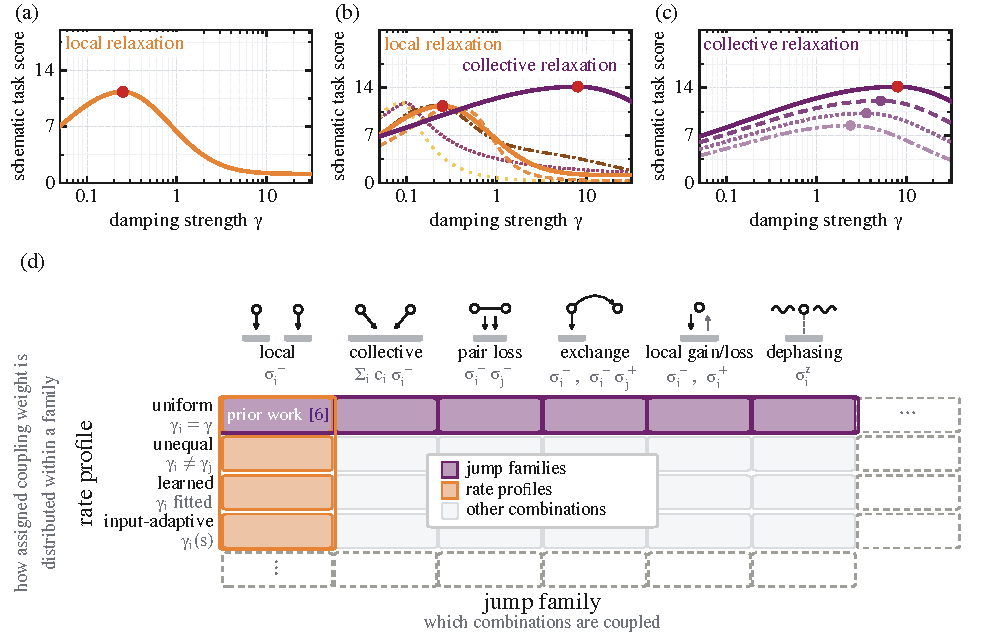
\includegraphics{figures/fig_designspace.pdf}};
% Figure-native PDF text cannot carry a manuscript-internal citation target
% through \includegraphics. This transparent, number-sized link sits exactly
% over the visible "6" in panel (d) and jumps to the Sannia et al. entry.
\begin{scope}[
  x={(designspacegraphic.south east)},
  y={(designspacegraphic.north west)}
]
\node[anchor=center,inner sep=0,outer sep=0] at (0.31685,0.34760)
  {\hyperlink{cite.Sannia2024}{\phantom{6}}};
\end{scope}
\end{tikzpicture}
\caption{\textbf{Dissipator geometry separates two complementary design
coordinates.}
\emph{(a)} Previous work primarily varies the overall strength of uniform
local relaxation~\cite{Sannia2024}. \emph{(b)} The jump family changes which
system combinations couple directly to the environment. \emph{(c)} The rate
profile redistributes coupling weight within a selected family.
\emph{(d)} Highlighted cells mark the two principal coordinate slices;
pale-gray cells show other combinations. Panels (a--c) show schematic task
scores, not fitted task data.}
\label{fig:space}
\end{figure*}

Figure~\ref{fig:space} maps these choices across the tested design space. The
local--collective example is intuitive, but the distinction must be defined at
the generator level.

Let \(\{F_\mu\}\) be a fixed set of traceless system operators with
\[
\Tr(F_\mu^\dagger F_\nu)=\delta_{\mu\nu}.
\]
Expanding every jump operator as
\[
L_k=\sum_\mu A_{k\mu}F_\mu,
\qquad
C=A^\dagger A\succeq0,
\]
makes this distinction invariant. The coefficient \(A_{k\mu}\) states how
strongly elementary action \(F_\mu\) contributes to environmental channel
\(k\). The matrix \(C\) records which elementary actions are coupled and how
the coupling weight is arranged among them. Equivalent remixings of the jump
list change the individual \(L_k\) and \(A\), but leave \(C\), and therefore
the dissipative generator, unchanged.
These coordinates are operational rather than globally orthogonal: a family
fixes the operator sector and allowed support of \(C\), whereas within-family
parameters set its nonzero weights and, where applicable, its direction within
that support. The construction is invariant under equivalent jump-list
remixings but remains relative to the declared elementary-operator basis.

For the one-body lowering block, the local--collective distinction takes the
form
\[
C_{\mathrm{lower}}^{\mathrm{local}}\propto I_N,
\qquad
C_{\mathrm{lower}}^{\mathrm{collective}}
  \propto \boldsymbol c\boldsymbol c^\dagger,
\]
where
\(\boldsymbol c=(c_1,\ldots,c_N)^{\mathsf T}\) parameterizes the shared
operator
\[
L_{\mathrm c}\propto\sum_i c_i\sigma_i^-.
\]
With nonzero local rates, \(I_N\) spans \(N\) independently coupled lowering
directions, whereas
\(\boldsymbol c\boldsymbol c^\dagger\) spans one directly coupled collective
direction. Rotating the written local jump operators cannot turn this
full-rank block into the rank-one shared block. Thus local and collective
relaxation are distinct generators.
\Needspace{3\baselineskip}
Unequal local relaxation instead changes the diagonal weights within the local
block and thus moves along the rate-profile axis.

\Needspace{4\baselineskip}
Table~\ref{tab:designs} is the exact catalogue of the tested environmental
actions; Fig.~\ref{fig:space} provides their intuitive map. We say gain/loss
rather than thermalization because its fixed transitions need not produce a
thermal state.

\subsection{Common structural normalization and paired comparison}

Unlike families contain different numbers and types of jump operators.
Assigning the same coefficient to every operator would therefore give more
total weight to a family merely because it contains more operators. We instead
fix
\begin{equation}
\mathcal B=\sum_k\Tr(L_k^\dagger L_k).
\label{eq:budget-intro}
\end{equation}
Each term is the squared operator size assigned to one environmental channel.
In the orthonormal basis above, \(\mathcal B=\Tr C\). Fixing
\(\mathcal B\) therefore provides a common structural bookkeeping scale: the
total assigned operator weight remains fixed while its organization changes.

For the principal fixed-\(\mathcal B\), common-protocol comparison, we vary
only the jump family. The Hamiltonian instance, input sequence, Pauli
observables, linear readout, training, selection, and test splits, and assigned
operator weight \(\mathcal B\) remain fixed.

This isolates structural change, not physical equivalence. In the one-body
local--collective comparison, fixed \(\mathcal B=\Tr C\) holds assigned coupling
weight fixed while changing the cross-site dissipative correlations encoded in
\(C\); it does not equalize activity,
the relaxation spectrum, energy flow, entropy production, implementation, or
hardware cost. The fixed-\(\mathcal B\) protocol therefore defines the cross-family
structural slice, while activity, gap, and operating-point controls additionally
validate only the local--collective memory ordering.

\subsection{Readout and computational tasks}

After each input interval, local Pauli expectations and same-axis two-qubit
correlations summarize the reservoir state,
\[
\{\langle X_i\rangle,\langle Y_i\rangle,\langle Z_i\rangle,
\langle X_iX_j\rangle,\langle Y_iY_j\rangle,\langle Z_iZ_j\rangle\}.
\]
They provide \(3N+3\binom{N}{2}\) features, or \(45\) at \(N=5\). Fixed-profile
structural experiments fit only the linear readout; separately identified profile and
operating-point studies also select dissipative parameters on data disjoint
from final testing. Appendix~\ref{app:experiment1} gives the ridge control.

Four benchmarks ask what information those features retain. Short-term memory
(STM)~\cite{JaegerSTM2001} reconstructs earlier inputs. NARMA-10
is the nonlinear autoregressive moving-average task of order ten. It tests a
nonlinear function of recent input history~\cite{AtiyaParlos2000}.
Parity combines binary memory with nonlinear processing. Mackey--Glass
forecasting~\cite{MackeyGlass1977} continues a chaotic signal in closed loop.
Capacity is maximized for STM and parity. Error is minimized for NARMA-10 and
forecasting.

For the adaptive-profile, finite-sampling, and alternative-control studies,
any additional mean matching, estimator choice, calibration, or selection
rule is stated explicitly.

\begin{table}[H]
\centering
\caption{\textbf{Dissipative designs.} The first two rows differ only in rate
profile. The displayed jump operators are convenient representatives of the
corresponding GKLS generators. Equivalent jump decompositions are not counted
as different designs.}
\label{tab:designs}
\footnotesize
\setlength{\tabcolsep}{3pt}
\renewcommand{\arraystretch}{1.06}
\begin{tabular}{@{}p{0.29\columnwidth}p{0.65\columnwidth}@{}}
\toprule
{\raggedright design\par}
& {\raggedright operators and direct environmental action\par}\tabularnewline
\midrule
{\raggedright\textbf{uniform local relaxation}~\cite{Sannia2024}\par}
& {\raggedright \(L_i=\sqrt{\gamma}\,\sigma_i^-\),
\(i=1,\ldots,N\). The same rate for every qubit; independent sitewise
relaxation and the reference design.\par}\tabularnewline
{\raggedright\textbf{unequal local relaxation}\par}
& {\raggedright \(L_i=\sqrt{\gamma_i}\,\sigma_i^-\),
\(i=1,\ldots,N\), with the \(\gamma_i\) not all equal. Independent sitewise
relaxation with qubit-dependent timescales.\par}\tabularnewline
\midrule
{\raggedright\textbf{collective relaxation}\par}
& {\raggedright \(\{\sum_i c_i\sigma_i^-\}\). One shared relaxation
channel.\par}\tabularnewline
{\raggedright\textbf{pair loss}\par}
& {\raggedright \(\{\sigma_i^-\sigma_j^-\}_{i<j}\). Joint two-excitation
removal.\par}\tabularnewline
{\raggedright\textbf{exchange-assisted relaxation}\par}
& {\raggedright
\(\{\sigma_i^-\}\cup\{\sigma_i^-\sigma_j^+\}_{i\ne j}\). Local lowering
supplemented by incoherent excitation exchange.\par}\tabularnewline
{\raggedright\textbf{local gain/loss}\par}
& {\raggedright \(\{\sigma_i^-,\sigma_i^+\}\). Fixed downward and upward
transitions.\par}\tabularnewline
{\raggedright\textbf{dephasing}\par}
& {\raggedright \(\{\sigma_i^z\}\). Phase randomization without excitation
loss.\par}\tabularnewline
\bottomrule
\end{tabular}
\end{table}
